\documentclass[tikz,border=2pt]{standalone}
\usepackage{amsmath}
\usetikzlibrary{arrows.meta}
\begin{document}
% Bag with 6 red and 4 blue balls, draw 3 without replacement, B = 10000 repetitions after
% set.seed(42): n_red starts 2 2 1 1, mean(n_red >= 2) = 0.6658, exact value 2/3.
\newcommand{\cellrow}[4]{% x0, y, colour, list of entries
  \foreach \v [count=\i from 0] in {#4} {\draw[#3, fill=#3!10] (#1+\i*0.95,#2) rectangle ++(0.95,0.5);
    \node[#3] at (#1+\i*0.95+0.475,#2+0.25) {\texttt{\v}};}}
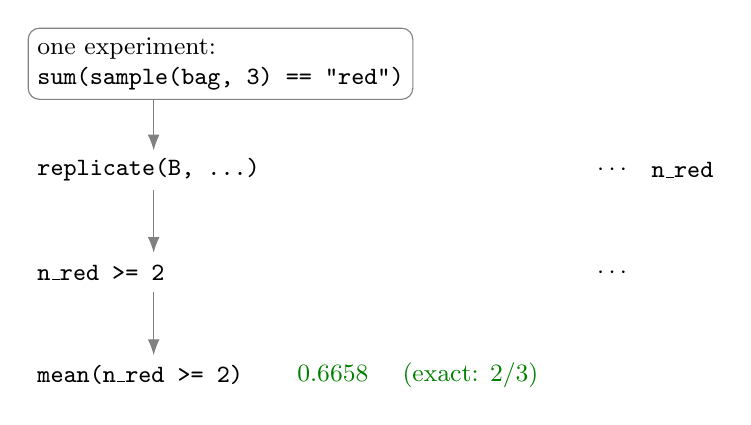
\begin{tikzpicture}[font=\small, >={Latex[length=2mm]}]
  % one experiment
  \node[draw=gray, rounded corners, align=left, anchor=west] (exp) at (0,0)
    {one experiment:\\\texttt{sum(sample(bag, 3) == "red")}};
  % replicate
  \node[anchor=west] at (0,-1.35) {\texttt{replicate(B, ...)}};
  \cellrow{3.3}{-1.6}{blue!70!black}{2,2,1,1}
  \node at (7.45,-1.35) {$\cdots$};
  \node[anchor=west] at (7.8,-1.35) {\texttt{n\_red}};
  \draw[->, gray] (1.6,-0.45) -- (1.6,-1.1);
  % comparison
  \node[anchor=west] at (0,-2.65) {\texttt{n\_red >= 2}};
  \cellrow{3.3}{-2.9}{red!70!black}{TRUE,TRUE,FALSE,FALSE}
  \node at (7.45,-2.65) {$\cdots$};
  \draw[->, gray] (1.6,-1.6) -- (1.6,-2.4);
  % mean
  \node[anchor=west] at (0,-3.95) {\texttt{mean(n\_red >= 2)}};
  \node[green!50!black, anchor=west] at (3.3,-3.95) {$0.6658$ \quad (exact: $2/3$)};
  \draw[->, gray] (1.6,-2.9) -- (1.6,-3.7);
\end{tikzpicture}
\end{document}
